\subsection{Background}
Traumatic Brain Injury (TBI) occurs from an impact to the head resulting in an injury to the brain, commonly caused by road traffic accidents and falls \cite{Langlois2006}. The severity of the injury sustained to the brain can range from superficial swelling to oedema and haematomas, with higher severity of the TBI resulting in a higher mortality rate as shown in Table~\ref{table:severity of TBI}. Even if the injury does not result in death, TBI can lead to long term disability and cognitive problems \cite{WorldHealthOrganisation2006}. Approximately 2.5 million people visited the hospital for TBI related symptoms in the US during 2013, of which 56,000 resulted in death \cite{Taylor2017}. The prevalence of this injury incurs an estimated \$60 billion cost annually to society to cover medical costs and lost productivity \cite{Finkelstein2009}. 

Primary TBI is the damage sustained from the initial impact, whereas secondary TBI occurs from the cascade of biochemical processes following from primary TBI, resulting in damage to the tissue surrounding the primary injury site \cite{Norton2008}. Secondary TBI tends to occur after a delayed period of time in about 30\%-40\% of cases, however whether it occurs is unpredictable and unpreventable \cite{Pagkalos2017}. Secondary effects, such as oedema, hypoxia and ischemia, can lead to neural degeneration and irreversible damage which can cause severe disability or be fatal \cite{Murthy2005}. Hence, it is crucial to diagnose secondary TBI as early as possible and provide appropriate medication to treat and minimise the damage.

\begin{table}[H]
\centering
\begin{tabular}{||c c||} 
 \hline
 Severity of TBI & Mortality (\%) \\ [0.5ex] 
 \hline\hline
 Mild & \textless 1 \\ 
 Moderate & 2-5 \\
 Severe & 20-50 \\
 \hline
\end{tabular}
\caption{Severity of TBI affecting mortality rates \cite{WorldHealthOrganisation2006}}
\label{table:severity of TBI}
\end{table}


When a patient is admitted with a head injury, common methods for prognosis include the Glasgow Coma Scale (GCS) \cite{WorldHealthOrganisation2006} and the Glasgow Outcome Scale (GOS) \cite{Jennett1975}, which use a scoring system based on the patient's physiological state. The GCS assesses ocular, motor, and verbal responses to assign the patient with a score out of 15 to determine the severity of TBI. The GOS categorises the patient into one of five categories that predicts the recovery of the patient. These methods are commonly accompanied with a neuroimaging of the brain to provide further information. The main disadvantage of these methods is that they are subjective, and it is difficult to identify mild symptoms of TBI which are displayed subtly as non-specific symptoms \cite{Bettermann2012}. Furthermore, these methods only capture information at a specific period in time meaning that if symptoms occur in between check ups, they will be unobserved until the next appointment. 

Prognostic models \cite{Steyerberg2008} have been developed from the IMPACT database \cite{Maas2007} that take into account several patient characteristics, such as age, hypotension, and haemoglobin levels, to predict the patient's outcome after six months using odds ratios. These high complexity models allow for clinicians to plan treatment based on the prognosis, however it is still not a method to diagnose a patient, merely predict the outcome. 

Early diagnosis is crucial for the best recovery, and to do so, there is a need to continuously monitor the patient and receive quantitative data in real time for accurate diagnosis. The Boutelle Research Group have been looking into utilising brain signals that are associated with TBI. From the primary injury site, spreading depolarisation (SD) waves \cite{Leao1944} propagate into surrounding brain tissue and cause secondary damage \cite{Brain2011}. Research has shown that monitoring SDs provides more information than routine clinical checkups \cite{Hartings2011}. A SD is characterised by the cells in the injury sites having a high energy demand to repolarise the membrane potential, hence the glucose concentration in the extracellular fluid transiently decreases by approximately 18-93$\mu M$. The cells tend to undergo anaerobic respiration during this period, so the extracellular lactate concentration transiently increase by 5-100$\mu M$ \cite{D.2010}. Glucose and lactate have been declared by the International Microdialysis Collaborative Group as the most clinically useful signals for the prognosis of TBI \cite{Hutchinson2015} so these transient changes are useful to monitor in high time resolution. Furthermore, during the same transient period, the potassium ion concentration increases \cite{Rogers2011} from 3$mM$ \cite{Katzman1976} to 30-50$mM$ \cite{Ayata2015} due to the cells depolarising. 


\begin{figure}[t!]
\centering
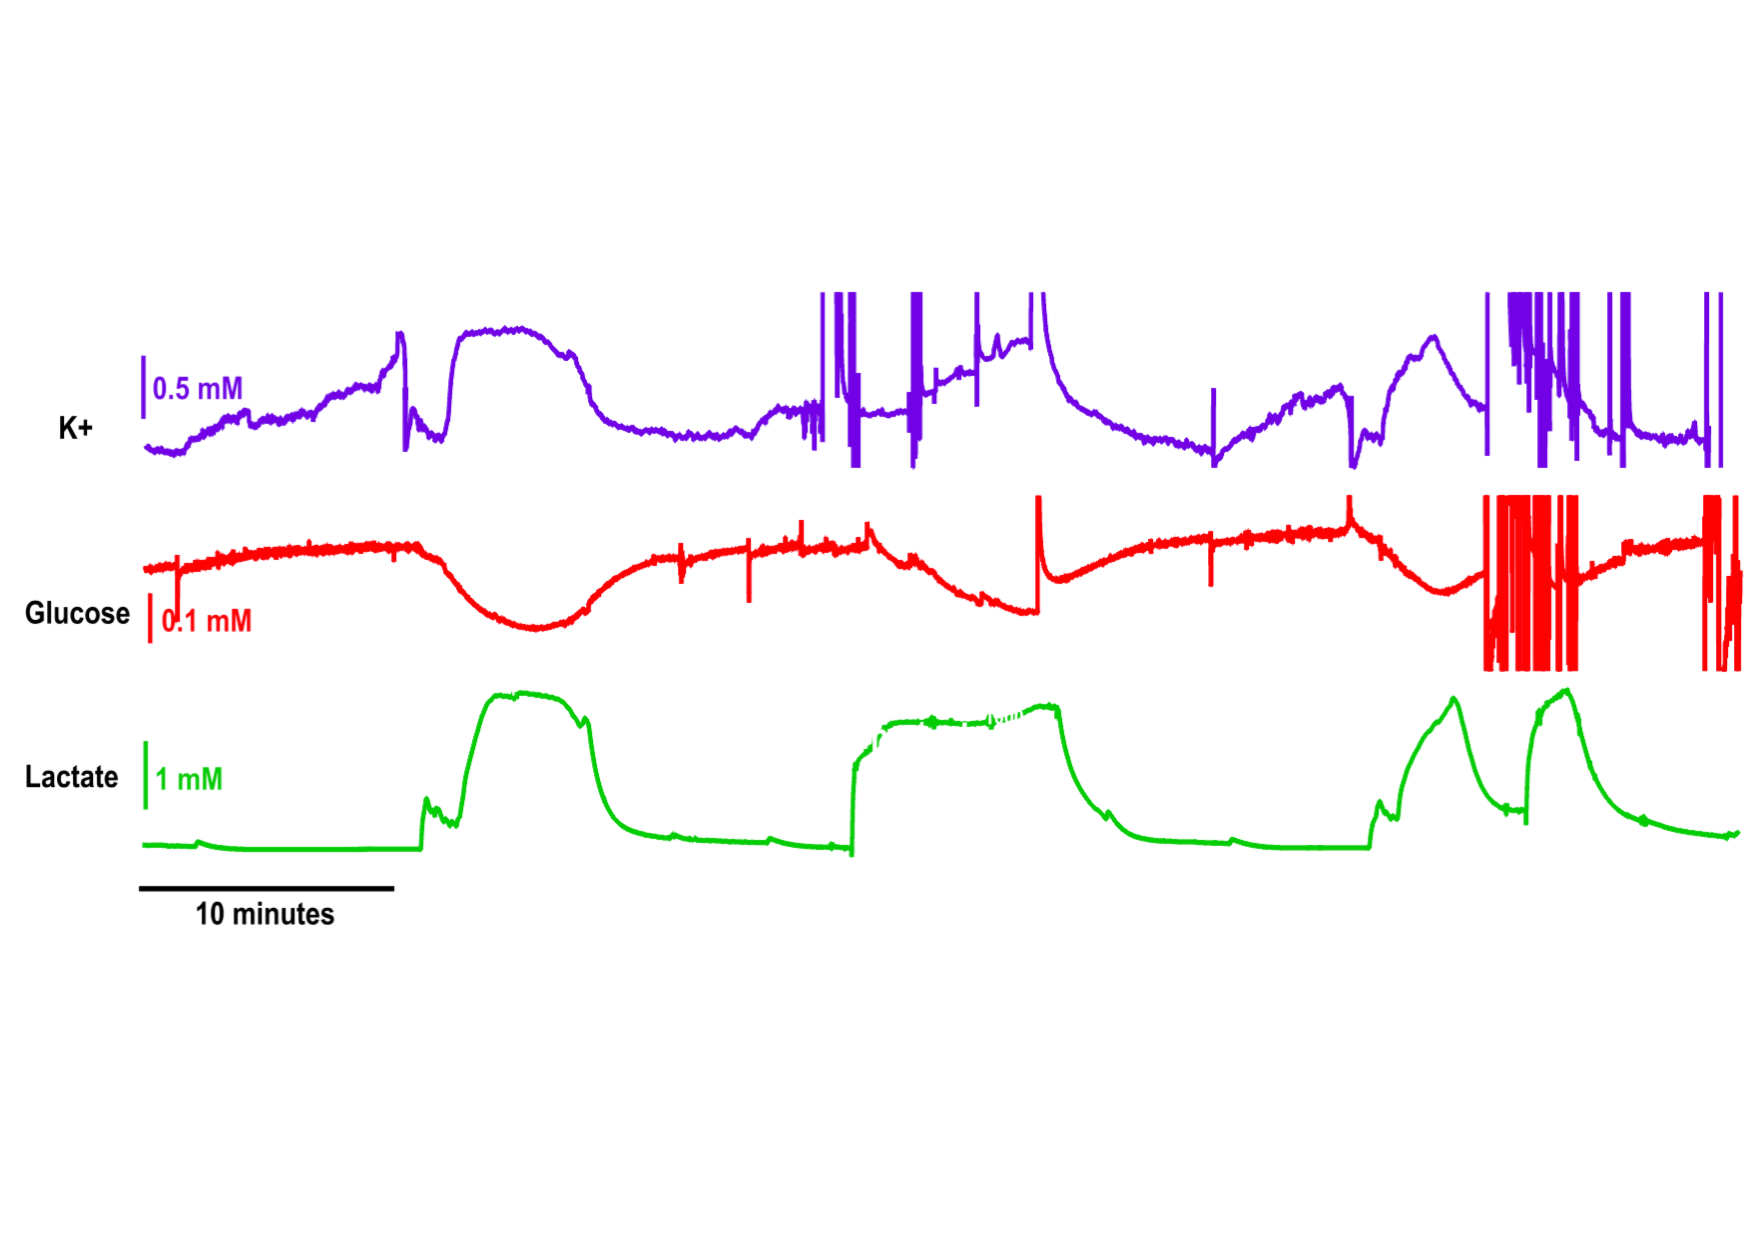
\includegraphics[trim={0cm 5cm 0.5cm  5cm}, clip, width=1\textwidth]{./figures/conc.pdf}
\captionsetup{justification=centering}
\caption{Biochemical changes during an SD occurence at 10 minutes. K+ and lactate show an increase in concentration whilst glucose shows a decrease in concentration \cite{Rogers2017}. Measurements obtained from continuous online microdialysis.}
\label{fig: SD}
\end{figure}

\subsection{Online Microdialysis System}
The research group have developed a novel monitoring system, a continuous online microdialysis (coMD), to monitor the neurochemical changes that occur during a SD wave with excellent temporal resolution. A miniaturised microdialysis probe is inserted on the surface of the brain and is perfused with sterile artificial cerebrospinal fluid (aCSF). The microdialysite then perfuses through a microfluidic chip that houses the three sensors that detect the glucose, potassium and lactate concentrations in the brain. This set up has allowed for online microdialysis monitoring and the transient changes in glucose, lactate and potassium to be accurately measured \cite{Rogers2017} as shown in Figure~\ref{fig: SD}.

To collect data from the patient, the microfluidic analysis system has to be placed behind the patient's bed on a trolley. The sensors were then wired into the Powerlab data acquistition (DAQ) hardware, which was then wired to a computer so that the measurements from the sensors could be viewed in real time on the associated software, PowerLab Pro \cite{Rogers2017}. This setup that the patient is attached to is very bulky and the wired system poses disadvantages such as restriction on the patient's movement, the wires may break or disconnect, and the wires may introduce noise \cite{Ferguson2011}. A more desirable system is one that is miniaturised and instead allows for wireless transmission of data.



\subsection{Aim}
This project aims to develop a wireless communication system between the coMD system and an iOS application. Information from the three electrochemical sensors will be received simultaneously in an iPad application in real time to allow for continuous monitoring of the patient in high temporal resolution. The app must be user friendly and be of high quality as it aims to be used by a clinician to monitor the state of the patient. It is desirable for the app to contain features that allows for easy use and easy readability of the data presented. It is important that the signals are transmitted and displayed accurately so suitable processing methods need to be implemented. 

